\documentclass[a0,landscape]{a0poster}

%\usepackage[landscape]{geometry}
\usepackage{amsthm,amssymb,amsmath}
\usepackage{float}
\usepackage{graphicx,xcolor}
\usepackage{listings}
\lstset{basicstyle=\ttfamily\large,basewidth=0.5em,mathescape}
\usepackage{multicol}
\usepackage{wrapfig,xspace}
\usepackage{url}
\def\latexml{{\LaTeX}ML\xspace}
\def\lec#1{\strut\hfil\strut\null\nobreak\hfill\hbox{(#1)}\par}
\usepackage{tikz}\usetikzlibrary{docicon}
\def\blue#1{\textcolor{blue}{#1}}

\begin{document}

\title{A Semantics-Aware {\LaTeX}-to-Office Converter}
\author{Lukas Kohlhase and Michael Kohlhase}
\institute{Jacobs University Bremen}
\email{https://latin.omdoc.org}

\abstract{We present a {\LaTeX}-to-Office conversion plugin for \latexml that can bridge
  the divide between publication practices in the theoretical disciplines (\LaTeX) and the
  applied ones (predominantly Office). The advantage of this plugin over other converters
  is that \latexml conserves enough of the document- and formula structure, that the
  transformed structures can be edited and processed further.}

\titlepage

\begin{multicols}{3}
\raggedright

\section*{Problem}\label{sec:intro}
\begin{itemize}
\item Technical documents from the STEM fields augment the text with structured objects --
  images, mathematical/chemical formulae, diagrams, and tables -- that carry essential
  parts of the information.
\item There are two camps with different techniques for
authoring documents. 
\begin{itemize}
\item theoretical disciplines (Mathematics, Physics, and CS) prefer {\LaTeX},
\item applied ones (e.g. Life Sciences, Chemistry,
Engineering) use Office Suites almost exclusively.
\end{itemize}
\item Transforming between these two document
formatting approaches is non-trivial:
\begin{itemize}
\item {\TeX/\LaTeX} uses in-document macros to ``program'' documents, empowering authors
  to automate document aspects ({\LaTeX} packages).
\item Office suites rely on document styles that adapt visual parameters.
\end{itemize}
each camp deems their approach vastly superior and the other's insufferable.
\item Problems in trans-paradigm collaboration. 
\end{itemize}

\section*{State of the Art \& Approach}
Three ways of transforming {\TeX/\LaTeX} to Office documents.\lec{converse direction
  different methods}
\begin{enumerate}
\item \textbf{copy/paste or import from PDF} There are two problems with this route:
\begin{itemize}
\item mathematical formulae are not preserved 
\begin{center}
  \begin{tabular}{|c|c|}\hline%|
    copy from PDF & paste (libreoffice)\\\hline
    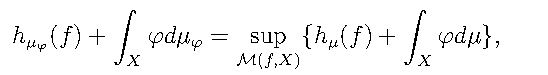
\includegraphics[width=17.5cm]{mathsnippet} & 
    
\includegraphics[width=17.5cm]{mathsnippet-libreoffice}\\\hline
  \end{tabular}\\
\textbf{Copy \& Paste in Word Processors}
\end{center}
\item even if the result looks OK the results have lost their links (e.g. for
  citations/references or label/ref), or become difficult to edit, because they do not
  conform to the styling system of the word processor.
\end{itemize}
\blue{Fundamental Problem}: Process only converts the appearance of the
document\lec{meaning is lost}
\item \textbf{Parsing \LaTeX sources, generating Office format}, e.g. \texttt{latex2rtf}
  (custom {\TeX} parser, incomplete) or \texttt{TeX4HT} (use {\TeX}, seed DVI, parse that,
  needs bindings).
\item \textbf{Our approach: Convert {\LaTex} to XML, transform this}: \latexml converts to
  XML conserving author-supplied semantics (given \latexml bindings)
\end{enumerate}

\section*{The Office Formats}\label{sec:target}

WML (MS Office) and ODT (Open/LibreOffice) follow the same architectural paradigm:
zip-packaged directories of XML files that contain document content, metadata, and
styling.

Math as external objects in StarOffice/MathML in ODT and as proprietary XML format in WML,
e.g. for  $1.5\times 10^7$: 
\lstinputlisting[basicstyle=\sf,language=XML]{wmlmath.xml}

\section*{Transformation}\label{sec:trans}

\begin{center}
\begin{tikzpicture}[yscale=1.5,xscale=1.5]
\tikzstyle{doc}=[draw,thick,align=center,color=black,
                 shape=document,minimum width=10mm,minimum height=7mm]
\node[doc] (p) at (-1,3.5) {\texttt{paper.tex}};
\node[doc] (b) at (1,3.5) {\texttt{group.bib}};
\node[doc,dashed] (px) at (-1,2.2) {\texttt{paper.tex.xml}};
\node[doc,dashed] (bx) at (1,2.67) {\texttt{group.tex.xml}};
\draw[->,thick] (p) -- node[left,near end] (l) {\latexml} (px);
\draw[->,thick] (b) -- (bx);
\draw[->,thick] (bx) -- (l);
\node[doc,dashed] (d) at (-2,1) {\texttt{document.xml}};
\node[doc,dashed] (r) at (0.2,1) {\texttt{relations.xml}};
\node[doc] (s) at (1,.3) {\texttt{styles.xml}};
\draw[->,thick] (px) -- node[left]{XSLT}(d);
\draw[->,thick] (px) -- node[right]{XSLT}(r); 
\node[inner sep=0pt,outer sep=0pt] (z) at (-1,.3) {};
\draw[thick] (d) -- (z);
\draw[thick] (r) -- (z);
\draw[thick] (s) -- (z);
\node[doc] (dx) at (0-1,-.4) {\texttt{paper.docx}};
\draw[->,thick] (z) -- node[left] {zip} (dx);
\draw[dotted] (-3.1,-.1) rectangle (1.9,1.9);
\node at (1.6,1.8) {post};
\end{tikzpicture}
\end{center}
The user does not see all these transformation, generation, and packaging steps: given a
{\LaTeX} paper, all she has to do is type
\begin{quote}\tt
latexmlc paper.tex --destination=paper.docx --profile=word
\end{quote}
\texttt{destination=paper.odt} gives ODT
\section*{Result: Converted Formula in MS Word}
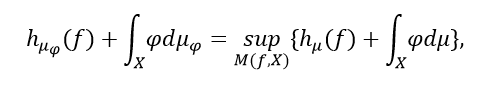
\includegraphics[width=30cm]{convertedmathsnippet}\\

\section*{Limitations}
\begin{enumerate}
\item we cannot currently generate the text-based input format (StarMath or the WML {\TeX}
  variant)\lec{further editing difficult}
\item conversion of citations and references into ``semantic'' formats partial
\end{enumerate}

\section*{Future Work}
\begin{enumerate}
\item For ODF formulae, use of the TeXMaths plugin for Libreoffice, which uses {\LaTeX}
  instead of StarMath for user input of formulae
\item develop an ``office package'' for \LaTeX and a corresponding \latexml binding, which
  allows the direct markup/transformation of higher-level structures.
\item extend the transformation to carry over even more semantics from the \stex format
  into semantically extended office formats like CPoint or CWord
\end{enumerate}

\section*{Availability}
Public Domain on Github: \url{https://github.com/KWARC/LaTeXML-Plugin-Doc}
\end{multicols}
\end{document}

%  LocalWords:  latexml titlepage multicols raggedright lec textbf hline libreoffice px
%  LocalWords:  includegraphics mathsnippet texttt lstinputlisting basicstyle wmlmath.xml
%  LocalWords:  tikzpicture yscale xscale tikzstyle bx paper.docx tt latexmlc paper.odt
%  LocalWords:  convertedmathsnippet TeXMaths stex CPoint CWord
